\chapter{Extending FLID}
\label{sec:models}

\section{Beyond Diversity: FLDC}

Diversity is an important property in the context of summarization \citep{tschiatschek16learning}, however it is not the only one. Coherence is also a desired property of summaries, particularly for structured summaries \citep{Yan:2011:ETS:2009916.2010016}. Balancing coherence and diversity is considered a challenge and maxiziming diversity alone may lead to disconnected summaries, while focusing on coherence can hinder the breadth of the resulting summaries \citep{Shahaf2012}.

To better understand why coherence is important, consider the construction of a spatial summary for photos taken in a city. A model based on spatial diversity would create sets containing photos taking at distant locations in the city, however another possibility is to have summaries that contain photos that were taken close to some starting point, in this case the desired property is not spatial diversity but rather coherence.

Therefore, a natural extension to the FLID model is to add the capacity of modeling coherence along with diversity. I propose the addition of a log-supermodular term analogous to the log-submodular term \eqref{eq:diversity} in order to model the complementarity between elements.

This supermodular term introduces a representation of the elements using $K$-dimensional vectors $\mathbf{w}^{K} \in \mathbb{R}^{K}_{\geq 0}$, where each dimension $1 \leq c \leq K$ captures a concept that relates to set coherence and $w_{i,c}$ quantifies the contribution of each element $i$ to each coherence concept $c$. The coherence of a set $S$ with respect to each concept $c$ is quantified as $\sum_{i \in S}{w^{e}_{i,c}} - \max_{i \in S}{w^{e}_{i,c}}$ which is a supermodular term mirroring the submodular term in FLID. Summing over all the concepts results in the proposed coherence term. Hereby, define $\mathbf{W}^{e} \in \mathbb{R}^{|V| \times K}_{\geq 0}$ as the matrix where the $i$-th row is the representation $\mathbf{w}^{e}$ of element $i$.

Adding the coherence term to FLID results in the extended model, which I refer to as the Facility Location Diversity and Coherence (FLDC) model. Its probability distribution is defined as:

\begin{equation}
  \tag{FLDC}
  P(S) = \frac{1}{Z}\exp{\left(\sum_{i \in S}{u_{i}} + \mathrm{div}(S) + \sum_{c=1}^{K}{\left(\sum_{i \in S}{w^{e}_{i,c}} - \max_{i \in S}{w^{e}_{i,c}}\right)}\right)}
  \label{eq:fldc}
\end{equation}

\subsection{Partition Function}

For the FLDC model, the partition function can be computed in $\mathcal{O}(|V|^{L+K+1})$ time. This complexity can be derived using a similar algorithm as the one presented by \citet{tschiatschek16learning} for FLID, the key observation is that the algorithm they present only requires the ordering of weights to determine elegible element for a set given a set of maximum weights per dimension, therefore this can be easily extented to include the the ordering for the coherence weights as well. This requires evaluating $K$ more dimensions which results in the added term to the exponent of the complexity expression, which makes the computation of the partition function more impractical than in the FLID case.

\subsection{Learning FLDC Models}

As with FLID, the parameters for an FLDC model can be estimated using NCE. For FLDC the vector $\boldsymbol{\theta}$ is composed of $[\mathbf{u}, \mathbf{W}^{b}, \mathbf{W}^{e}, \hat{Z}]$ and its gradient is the same as in equations \eqref{eq:gradient-flid-1}-\eqref{eq:gradient-flid-4} with the addition of a gradient with respect to the new parameter, $\mathbf{W}^{e}$, which is given by:

\begin{equation}
\left(\nabla_{\mathbf{W}^{e}}\log{\hat{P}_{d}(S; \hat{Z}, \mathbf{u}, \mathbf{W}^{e}, \mathbf{W}^{e})}\right)_{i,c} = \begin{cases}
1 & \text{if}\ i \in S\ \text{and}\ i \neq \argmax_{j \in S}{w^{e}_{j,c}} \\
0 & \text{otherwise}
\end{cases} \label{eq:sub-fldc}\\
\end{equation}

Where $\left(\nabla_{\mathbf{W}^{e}}\cdot \right)_{i,c}$ represents the $(i,c)$-th entry in the gradient with respect to $\mathbf{W}^{e}$.

This also affects the overall complexity of the learning algorithm. Computing the gradient takes $\mathcal{O}(L+K)|S|$ for FLDC at each step, therefore the running time of a full pass over the data and noise samples takes $\mathcal{O}(|\mathcal{D}\cup\mathcal{N}|\kappa(L+K))$. This is not significantly more expensive than learning FLID under the assumption that $K \simeq L$.


\subsection{Example: Two Non-overlapping Clusters}
\label{sec:fldc-toy}

As an example of the extended model, consider the distribution presented in table \ref{tab:fldc-toy-probs} for $V = \{1,2,3,4\}$, representing a set of two non-overlapping clusters with 2 elements each. Intuitively, this can be modeled by considering that there is diversity between elements in different clusters while inside a cluster there is a coherence component that ties them together.

Concretely, the weight matrices $\mathbf{W}^{b}, \mathbf{W}^{e}$ in Figure \ref{fig:fldc-toy-mixed-weights} illustrate one possible instance of the model. The corresponding utility vector is $\mathbf{u} = \overrightarrow{0}$, because there is no indication that an individual element is favored over the pairs. This model is easily interpretable and accurately realizes the distribution.

\begin{table}
  \centering
  \caption{Probability distribution for Example \ref{sec:fldc-toy}.}
  \begin{tabular}{@{}ll@{}}
    \toprule
    $S$ & $P(S)$  \\
    \midrule
    $\{1,2\}$ & $0.5$ \\
    $\{3,4\}$ & $0.5$ \\
    Otherwise & $0.0$ \\
    \bottomrule
  \end{tabular}
  \label{tab:fldc-toy-probs}
\end{table}

\begin{figure}
  \centering
  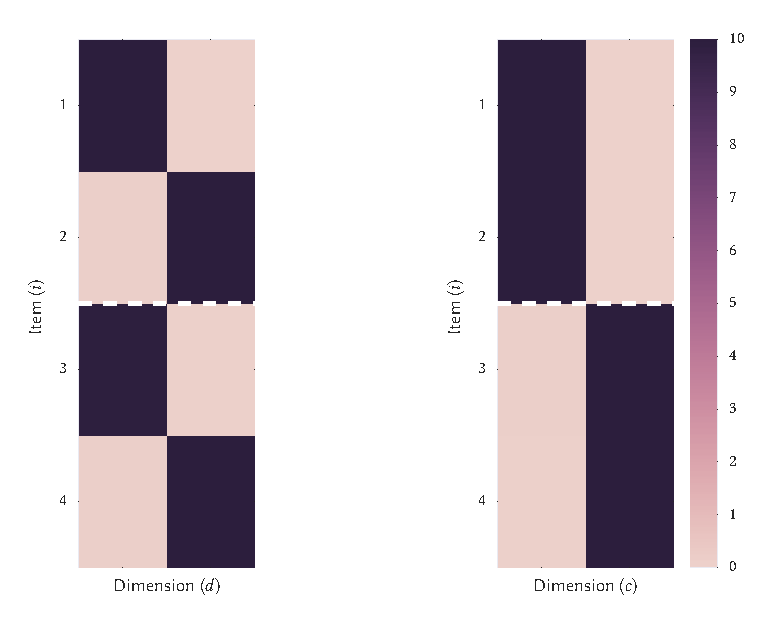
\includegraphics[width=\textwidth]{fldc_toy_example_mixed_weights}
  \caption{Diversity and coherence weights for FLDC model in Example \ref{sec:fldc-toy}. The dotted line divides the clusters.}
  \label{fig:fldc-toy-mixed-weights}
\end{figure}

\section{Generalizing through Features: FFLDC}

An important characteristic of the FLID model, and by extension the FLDC one, is that it is agnostic to the type of elements in the ground set, this allows its application to a wide range of problems without prior knowledge. However the downside is that the model has no capability to make use of information about the elements, if available, to improve the modeling of the data. Moreover, if a new element is added to the set there is no way to generalize the existing knowledge about similar elements.

In order to solve these problems, I propose a further extension to the model. Firstly, an element ($i \in V$) is represented as a vector $\mathbf{x}_{i} \in \mathbb{R}^{M}$ where each entry is a feature, e.g. for venues one feature could be its aggregated rating while another indicates whether it is indoors or outdoors. The representations of all elements is collected by matrix $\mathbf{X} \in \mathbb{R}^{|V| \times M}$ where each row $i$ corresponds to the repreesntation $\mathbf{x}_{i}$ of element $i$.

Then, the utility vector $\mathbf{u}$ and weight matrices $\mathbf{W}^{b}, \mathbf{W}^{e}$ are factorized to include this feature matrix $\mathbf{X}$ as follows:

\begin{align}
  \mathbf{u} &= \mathbf{Xa}   \label{eq:ffldc-factorization-1} \\
  \mathbf{W}^{b} &= \mathbf{XB}  \label{eq:ffldc-factorization-2} \\
  \mathbf{W}^{e} &= \mathbf{XE}
  \label{eq:ffldc-factorization-3}
\end{align} 

Where $\mathbf{a} \in \mathbb{R}^{M}$ represents the contribution of each feature to the total utility of an item, while $\mathbf{B} \in \mathbb{R}^{M \times L}$ and $\mathbf{E} \in \mathbb{R}^{M \times K}$ encode the contribution of each feature to each latent diversity and coherence dimension, respectively. The intuition behind this factorization is that the information about the items can enhance the latent representations, hence producing a richer model. For example if $M < |V|$ and the features are sufficient to represent the items, it is expected that learning will be easier because of the reduced number of parameters with respect to learning the equivalent FLDC model.

I refer to the extended model as the Featurized Facility Location Diversity and Coherence (FFLDC) model and its probability distribution is defined as:

\begin{align}
  \tag{FFLDC} \label{eq:ffldc}
  P(S) &= \frac{1}{Z}\exp{\left(\sum_{i \in S}{\sum_{k=1}^{M}x_{i,k}a_{k}} + fdiv(S) + fcoh(S)\right)} \\
  fdiv(S) &= \sum_{d=1}^{L}{\left(\max_{i \in S}{\sum_{k=1}^{M}x_{i,k}b_{k,d}} - \sum_{i \in S}{\sum_{k=1}^{M}x_{i,k}b_{k,d}}\right)} \\
  fcoh(S) &= \sum_{c=1}^{K}{\left(\sum_{i \in S}{\sum_{k=1}^{M}x_{i,k}e_{k,c}} - \max_{i \in S}{\sum_{k=1}^{M}x_{i,k}e_{k,c}}\right)}
\end{align}

Where $a_{i}$ is the $i$-th entry of $\mathbf{a}$, $b_{k,d}$ is the $(k,d)$-th entry of $\mathbf{B}$, $e_{k,d}$ is the $(k,e)$-th entry of $\mathbf{E}$ and $x_{i,k}$ is the $(i,k)$-th entry of $X$.

\begin{remark}
  If $\mathbf{X} = \mathcal{I}$, then FFLDC is equivalent to FLDC, with $\mathbf{a} = \mathbf{u}$, $\mathbf{W}^{b} = \mathbf{B}$ and $\mathbf{W}^{e} = \mathbf{E}$.
\end{remark}

The use of features also allows the application of the model to previously unseen elements, hence solving the aforementioned problem of generalization. This is possible because the model is defined on the space of features and not items, and for a previously unseen element $j$ only its representation $\mathbf{x}_{j}$ is required in order to evaluate the probability of sets containing this element.

\subsection{Partition Function}

The computation of the partition function for this model can be done using the fact that any FFLDC model can be transformed into an equivalent FLDC model through the factorizations in equations \eqref{eq:ffldc-factorization-1}-\eqref{eq:ffldc-factorization-3}. This transformation requires $\mathcal{O}(|V|M(L+K))$ time for the matrix multiplications, therefore the overall complexity of calculating the partition function for an FFLDC model is $\mathcal{O}(|V|M(L+K) + |V|^{L+K+1})$. This expression can be simplified to $\mathcal{O}(|V|^{L+K+1})$ because the exponential term is significantly larger assuming sensible values for $M$. Given that the complexity of computing the partition function for FFLDC is equivalent to the FLDC model, it is also intractable in practice.

\subsection{Learning FFLDC Models}

For FFLDC, the parameter vector $\boldsymbol{\theta}$ is different from the previous models, it is composed by $[\mathbf{a}, \mathbf{B}, \mathbf{C}, \hat{Z}]$ and the gradient of the NCE objective $g(\boldsymbol{\theta})$ is given by:

\begin{align}
  \left(\nabla_{\mathbf{a}}\log{\hat{P}_{d}(S; \hat{Z}, \mathbf{a}, \mathbf{B}, \mathbf{E})}\right)_{m} &= \sum_{i \in S} x_{i,m} \label{eq:sub-a}\\
  \left(\nabla_{\mathbf{B}}\log{\hat{P}_{d}(S; \hat{Z}, \mathbf{a}, \mathbf{B}, \mathbf{E})}\right)_{m,d} &= x_{i^{d},m} - \sum_{i \in S} x_{i,m} \label{eq:sub-b} \\
  \left(\nabla_{\mathbf{E}}\log{\hat{P}_{d}(S; \hat{Z}, \mathbf{a}, \mathbf{B}, \mathbf{E})}\right)_{m,c} &= x_{i^{c},m} - \sum_{i \in S} x_{i,m} \label{eq:sub-e}
\end{align}

Where $i^{d} = \argmax_{i \in S}{\sum_{k=1}^{M}{x_{i,k}b_{k,d}}}$ and $i^{c} = \argmax_{i \in S}{\sum_{k=1}^{M}x_{i,k}e_{k,c}}$. $\left(\nabla_{\mathbf{a}}\cdot \right)_{m}$ represents the $m$-th entry of the sub-gradient with respect to $a$, $\left(\nabla_{\mathbf{B}}\cdot\right)_{m,d}$ represents the $(m,d)$-th entry of the sub-gradient with respect to $B$ and $\left(\nabla_{\mathbf{E}}\cdot\right)_{m,c}$ represents the $(m,c)$-th entry of the sub-gradient with respect to $E$.

\begin{remark}
  For $\mathbf{X} = \mathcal{I}$, the sub-gradients in \ref{eq:sub-a}-\ref{eq:sub-e} are equivalent to the FLDC sub-gradients. Because $x_{i,m} = 1$ only when $i = m$.
\end{remark}

Regarding running time complexity, the FFLDC model requires more operations for the gradient due to the inclusion of features. Concretely, computing the gradient for a set $S$ takes $\mathcal{O}(|S|M(L+K))$ which makes the running time of a single pass over data and noise samples $\mathcal{O}(|\mathcal{D}\cup\mathcal{N}|M(L+K)\kappa)$. Even though this is larger than the complexity of FLID or FLDC, it is still linear on the data.

\subsection{Example: Rated Locations}
\label{sec:ffldc-toy}

A small town has 6 popular locations, each of them has been rated from 0 to 5, where 0 represents a bad review and 5 an excellent review. Collected data shows that a typical visitor is more likely to visit and take photos at places with high ratings, however this is not the only factor driving their behavior. For example, an average visitor does not visit two places that serve food on the same day instead the data shows that visitors usually go to one place that serves food and then to an outdoor one, or they just visit one that has both characteristics. This data is summarized in Table \ref{tab:ffldc-toy-probs}, the task is to model this behavior using the FFLDC model.

\begin{table}
  \centering
  \caption{Synthetic data for Example \ref{sec:ffldc-toy}.}
  \begin{tabular}{@{}ll@{}}
    \toprule
    Locations visited $(S)$ & $P(S)$  \\
    \midrule
    $\{1,3\}$ & $0.30$ \\
    $\{3,4\}$ & $0.25$ \\
    $\{3,6\}$ & $0.15$ \\
    $\{2\}$ & $0.10$ \\
    $\{1\}$ & $0.06$ \\
    $\{3\}, \{4\}$ & $0.04$ \\
    $\{5\}, \{6\}$ & $0.03$ \\
    Otherwise & $0.00$ \\
    \bottomrule
  \end{tabular}
  \label{tab:ffldc-toy-probs}
\end{table}

In this example there is knowledge about the items and what features are relevant for the data. These features are summarized in equation \eqref{eq:ffldc-toy-feats}. The first column corresponds to the aforementioned rating, the second and third are binary features indicating whether the location is an outdoor one and whether it serves food, respectively.

\begin{equation}
  \mathbf{X} = \left(
    \begin{array}{ccc}
      4 & 1 & 0 \\
      4 & 1 & 1 \\
      3 & 0 & 1 \\
      3 & 1 & 0 \\
      2 & 1 & 1 \\
      2 & 1 & 0  \\
     \end{array}
  \right)
  \label{eq:ffldc-toy-feats}
\end{equation}

A possiblity is an FFLDC model that encourages diversity on the second a third feature, i.e. models the idea that visitors do not go to more than one place that serves food or is outdoor, while assigning a positive utility and coherence value to the first feature, i.e. modeling the preference for places with high ratings. One such model is presented in Figure \ref{fig:ffldc-toy-all-weights}, this approximates distribution from Table \ref{tab:ffldc-toy-probs} and illustrates the type of model that is useful in this example.

\begin{figure}
  \centering
  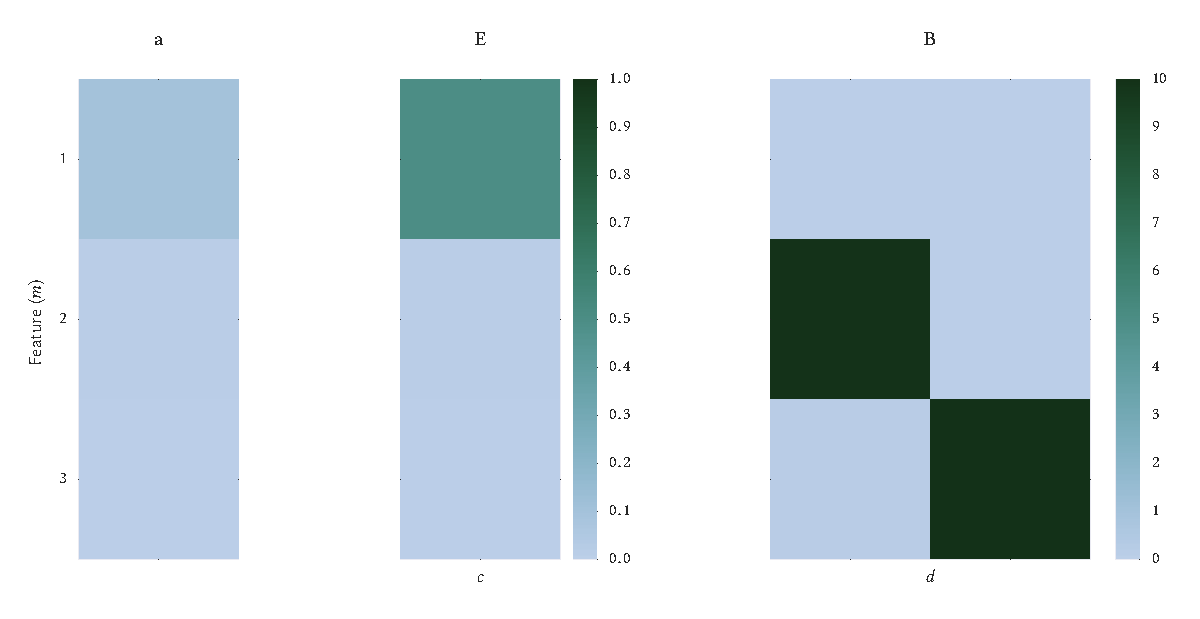
\includegraphics[width=\textwidth]{ffldc_toy_example}
  \caption{FFLDC sample model for Example \ref{sec:ffldc-toy}.}
  \label{fig:ffldc-toy-all-weights}
\end{figure}

If a new location $j$ is considered then it is possible to apply the model and estimate the probability of sets that include it. For example, consider a seventh location with the following features $\mathbf{x}_{7} = [5, 1, 0]$, using the same model parameters a new distribution can be computed without changing the model parameters, as it would be the case with FLID or FLDC. The updated distribution is shown in Table \ref{tab:ffldc-toy-probs-2} and it can be considered a sensible distribution given the problem description and the high rating of the new location, hence showing the model's capacity to generalize.

\begin{table}
  \centering
  \caption{Synthetic data for Example \ref{sec:ffldc-toy} after adding a new item.}
  \begin{tabular}{@{}ll@{}}
    \toprule
    Locations visited $(S)$ & $P(S)$  \\
    \midrule
    $\{3,7\}$ & $0.24$ \\
    $\{1,3\}$ & $0.21$ \\
    $\{3,4\}$ & $0.19$ \\
    $\{3,6\}$ & $0.10$ \\
    $\{7\}$ & $0.06$ \\
    $\{1\}, \{2\}$ & $0.04$ \\ 
    $\{3\}, \{4\}$ & $0.03$ \\
    $\{5\}, \{6\}$ & $0.02$ \\
    Otherwise & $0.00$ \\
    \bottomrule
  \end{tabular}
  \label{tab:ffldc-toy-probs-2}
\end{table}